\documentclass[11pt]{article}
\usepackage[utf8]{inputenc}
\usepackage[T1]{fontenc}
\usepackage[spanish]{babel}
\usepackage{times}
\usepackage{anysize}
\usepackage{verbatim}
\usepackage{float}
\usepackage{booktabs} % To thicken table lines

%%% TABLAS
\usepackage{tabularx}
\newcolumntype{b}{X}
\newcolumntype{B}{>{\hsize=.5\hsize}X}
\newcolumntype{s}{>{\hsize=.14\hsize}X}

%%%%%%%%%%%%%%%%%%%%%%%%%%%%%%%%%%% PARA CODIGO %%%%%%%%%%%%%%
\usepackage{color}
\definecolor{gray97}{gray}{.97}
\definecolor{gray75}{gray}{.75}
\definecolor{gray45}{gray}{.45}

\usepackage{listings}
\lstset{ frame=Ltb,
framerule=0pt,
aboveskip=0.5cm,
framextopmargin=3pt,
framexbottommargin=3pt,
framexleftmargin=0.4cm,
framesep=0pt,
rulesep=.4pt,
backgroundcolor=\color{gray97},
rulesepcolor=\color{black},
%
stringstyle=\ttfamily,
showstringspaces = false,
basicstyle=\small\ttfamily,
commentstyle=\color{gray45},
keywordstyle=\bfseries,
%
numbers=left,
numbersep=15pt,
numberstyle=\tiny,
numberfirstline = false,
breaklines=true,
}

% minimizar fragmentado de listados
\lstnewenvironment{listing}[1][]
{\lstset{#1}\pagebreak[0]}{\pagebreak[0]}

\lstdefinestyle{consola}
{basicstyle=\scriptsize\bf\ttfamily,
backgroundcolor=\color{gray75},
}

\lstdefinestyle{J}
 {language=Java,
 firstnumber=0,
 }
\lstdefinestyle{T}
{language=Haskell,
}

%\begin{lstlisting}[style=C]
%%codigo
%\end{lstlisting} 
%%%%%%%%%%%%%%%%%%%%%%%%%%%%%%%%%%% PARA CODIGO %%%%%%%%%%%%%%

%% Margenes
\marginsize{3cm}{2cm}{2cm}{2cm}

%Portada
\title{\textbf{\huge{Compilador de lenguaje de reglas para TORCS}}}
\author{Alejandro Trujillo Caballero}
\date{30 de junio de 2015}

\usepackage{graphicx}
\begin{document}

\maketitle
\thispagestyle{empty}
\newpage

\tableofcontents
\newpage

\section{Introducción}

El objetivo de esta práctica es la creación de un compilador que a partir de un lenguaje de reglas genere código Java
capaz de funcionar como un controlador de un piloto del simulador de carreras TORCS.


Para ello se analizará la especificación léxica y sintáctica del lenguaje, asi como su semántica y de forma escalonada se
codificarán cada una de las partes del compilador: analizador léxico, sintáctico, semántico, generación del árbol de sintaxis abstracta
y por último generación de código Java.

\section{Analizador Léxico}
\subsection{Especificación léxica}
El lenguaje incluye un total de 39 palabras reservadas:
perception, action, rules, inner, int, double, boolean, true, false, speed, angle, position, rpm, sensor0, sensor1 ... sensor18, gear, accelerate, brake, steering, if, else y while.

Caracteres especiales y operadores:

\medskip
\begin{table}[H]
\caption{Elementos sintácticos del lenguaje}
\begin{tabularx}{\textwidth}{Bb}
Función & Operador\\ \hline \hline
Separadores &  \{ \hspace{0.5cm} \} \hspace{0.5cm} -> \hspace{0.5cm} , \hspace{0.5cm} ; \hspace{0.5cm} ) \hspace{0.5cm} ( \\ \hline
Operadores aritméticos & + \hspace{0.5cm} - \hspace{0.5cm} * \hspace{0.5cm} / \hspace{0.5cm} \% \\ \hline
Operadores lógicos & \& \hspace{0.5cm} | \hspace{0.5cm} ! \hspace{0.5cm} \\ \hline
Operadores relacionaes & < \hspace{0.5cm} >  \hspace{0.5cm} <= \hspace{0.5cm} >= \hspace{0.5cm} <> \hspace{0.5cm} =\\ \hline
Asignación &  <- \\ \hline
Comentario & \# \\
\end{tabularx}
\end{table}

Los identificadores y literales se definen como:

\medskip
\begin{table}[H]
\caption{Identificadores y Literales}
\begin{tabularx}{\textwidth}{Bb}
Elemento & Expresión regular\\ \hline \hline
Identificadores & [\_ | [a-z] | [A-Z]] ( [\_| [a-z] | [A-Z] | [0-9]] )*  \\ \hline
Enteros & [1-9] [0-9]* \\ \hline
Double &  [0 | [1-9][0-9]*].[0-9]+  \\
\end{tabularx}
\end{table}

\subsection{Autómata finito determinista}

A continuación se encuentran los diagramas del autómata por el que se rige la máquina discriminadora determinista
del analizador léxico:

\begin{figure}[H]
\centering
\includegraphics[width=0.5\textwidth]{./DiagramasAutomata/img/BlancosYComentarios.png}
\caption{Blancos y comentarios.} \label{fig:blancosycomentarios}
\end{figure}

Estado final 2: Fin de comentario.

Estado final 3: Espacio blanco.

\begin{figure}[H]
\centering
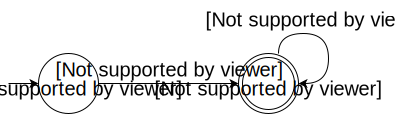
\includegraphics[width=0.5\textwidth]{./DiagramasAutomata/img/Identificadores.png}
\caption{Identificadores.} \label{fig:ident}
\end{figure}

Estado final 4: Identificador. Antes de lanzar el token de identificador, se comprueba si el lexema reconocido pertenece a
una palabra reservada, en caso de que sea así se utilizará el token de palabra reservada en su lugar.

\begin{figure}[H]
\centering
\includegraphics[width=0.5\textwidth]{./DiagramasAutomata/img/NumerosBueno.png}
\caption{Constantes numéricas.} \label{fig:números}
\end{figure}

Estado final 5: Número entero.

Estado final 6: Cero.

Estado final 8: Número decimal (Double).

\begin{figure}[H]
\centering
\includegraphics[width=0.5\textwidth]{./DiagramasAutomata/img/separadoresBueno.png}
\caption{Separadores.} \label{fig:sepa}
\end{figure}

Estado final 9: Apertura de llave.

Estado final 10: Cierre de llave.

Estado final 11: Apertura de parentesis.

Estado final 12: Cierre de parentesis.

Estado final 13: Separador coma.

Estado final 14: Separador punto y coma.

Estado final 15: Operador arirmético menos.

Estado final 16: Separador flecha.

\begin{figure}[H]
\centering
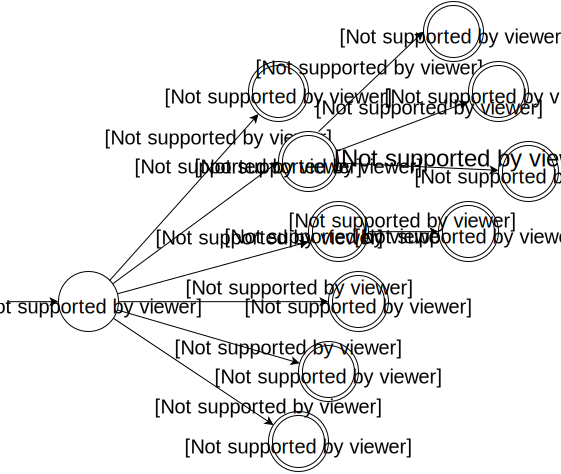
\includegraphics[width=0.5\textwidth]{./DiagramasAutomata/img/OperadoresLogYAsig.png}
\caption{Operadores lógicos y de asignación.} \label{fig:Log}
\end{figure}

Estados finales 17-25: Operadores relacionales o lógicos.

Estado final 26: Operador de asignación.


\begin{figure}[H]
\centering
\includegraphics[width=0.5\textwidth]{./DiagramasAutomata/img/OperadoresAritmBueno.png}
\caption{Operadores aritméticos.} \label{fig:aritm}
\end{figure}

Estados finales 27-30: Operadores aritméticos.

\subsection{Código del analizador léxico}

El código del analizador sigue la misma estructura que el del lenguaje Tinto en la práctica dos de la asignatura.

Las clases que lo implementan son: TORCSLexer y TokenConstants adjuntas (junto con el resto del código) a esta memoria.


\section{Analizador sintáctico}

\subsection{Gramática y conjuntos de predicción}

A continuación se muestra una tabla con la gramática LL(1) generada para el analizador junto con los conjuntos de primeros,
 siguientes y predicción de cada regla.

 Esta misma tabla también se encuentra en un archivo de hoja de cálculo adjunto a esta memoria por si por cuestiones de
 comodidad se desea (se recomienda) consultar en él.

 %TODO gramatica


 % Table generated by Excel2LaTeX from sheet 'Sheet1'
 \begin{table}[H]
   \centering
   \caption{Gramática LL(1) que describe el lenguaje.}
     \begin{tabularx}{\textwidth}{BBBBB}
     \toprule
     Simbolo & Regla & PRIMEROS & SIGUIENTES & PREDICCION \\
     \midrule
           &       &       &       &  \\
     Controller & ListDeclaration Rules & inner, perception, action, rules & \$    & inner, perception, action, rules \\
     ListDeclaration & Declaration ListDeclaration & inner, perception, action & rules & inner, perception, action \\
     ListDeclaration & lambda & lambda & rules & rules \\
           &       &       &       &  \\
     Declaration & InnerDecl & inner & inner, perception, action, rules & inner \\
     Declaration & PerceptionDecl & perception & inner, perception, action, rules & perception \\
     Declaration & ActionDecl & action & inner, perception, action, rules & action \\
           &       &       &       &  \\
     InnerDecl & inner Type identifier assing Literal semicolon & inner & inner, perception, action, rules & inner \\
     Type  & int   & int   & identifier & int \\
     Type  & char  & char  & identifier & char \\
     Type  & double & double & identifier & double \\
           &       &       &       &  \\
     PerceptionDecl & perception identifier ArgumentDecl PerceptionBody & perception & inner, perception, action, rules & perception \\
     ActionDecl & action identifier ArgumentDecl ActionBody & action & inner, perception, action, rules & action \\
     ArgumentDecl & lparen ListArguments rparen & lparen & lbrace & lparen \\
     ListArguments & Argument MoreArguments & int, char, double & rparen & int, char, double \\
     ListArguments & lambda & lambda & rparen & rparen \\
     MoreArguments & comma Argument MoreArguments & comma & rparen & comma \\
     MoreArguments & lambda & lambda & rparen & rparen \\
     Argument & Type identifier & int, char, double & comma, rparen & int, char, double \\
           &       &       &       &  \\
     PerceptionBody & lbrace ListPcptStatement rbrace & lbrace & perception & lbrace \\
     ListPcptStatement & PcptStatement ListPcptStatement & int, char, double, identifier, if, while, true, false, lbrace & rbrace & int, char, double, identifier, if, while, true, false, lbrace \\
     ListPcptStatement & lambda & lambda & rbrace & rbrace \\


     \bottomrule
     \end{tabularx}%
   \label{tab:gramatica}%
 \end{table}%

%%%%%%%%%%%%%%%%%%%%%%%%%%%%%%%%%%%%%%%%%%%%%%%%% oK %%%%
     \begin{tabularx}{\textwidth}{BBBbB}
     \toprule
     Simbolo & Regla & PRIMEROS & SIGUIENTES & PREDICCION \\
     \midrule
          &       &       &       &  \\
         ActionBody & lbrace ListActStatement rbrace & lbrace & inner, perception, action, rules & lbrace \\
     ListActStatement & ActStatement ListActStatement & int, char, double, identifier, **ConjuntoOutputs, if, while, lbrace & rbrace & int, char, double, identifier, **ConjuntoOutputs, if, while, lbrace \\
     ListActStatement & lambda & lambda & rbrace & rbrace \\
           &       &       &       &  \\
     Rules & rules lbrace ListRules rbrace & rules & \$    & rules \\
     ListRules & Rule ListRules & not, minus, plus, integer\_literal, double\_literal, true, false, identifier, lparen, **conjuntoInputs & rbrace & not, minus, plus, integer\_literal, double\_literal, true, false, identifier, lparen, **conjuntoInputs \\
     ListRules & lambda & lambda & rbrace & rbrace \\


     PcptStatement & PcptDecl & int, char, double & int, char, double, identifier, if, while, true, false, lbrace, rbrace & int, char, double \\
     PcptStatement & PcptAssignStm & identifier & int, char, double, identifier, if, while, true, false, lbrace, rbrace & identifier \\
     PcptStatement & PcptIfStm & if    & int, char, double, identifier, if, while, true, false, lbrace, rbrace & if \\
     PcptStatement & PcptWhileStm & while & int, char, double, identifier, if, while, true, false, lbrace, rbrace & while \\
     PcptStatement & PcptTrueStm & true  & int, char, double, identifier, if, while, true, false, lbrace, rbrace & true \\
     PcptStatement & PcptFalseStm & false & int, char, double, identifier, if, while, true, false, lbrace, rbrace & false \\
     PcptStatement & PcptBlockStm & lbrace & int, char, double, identifier, if, while, true, false, lbrace, rbrace & lbrace \\
           &       &       &       &  \\
     PcptDecl & Type identifier OptAssign semicolon & int, char, double & int, char, double, identifier, if, while, true, false, lbrace, rbrace & int, char, double \\

     \bottomrule
     \end{tabularx}%

%%%%%%%%%%%%%%%%%%%%%%%%%%%%%%%%%%%%%%%%%%%%%%%%%%%%%%%%%%%%%%%%%ok

\begin{tabularx}{\textwidth}{BBBBB}
          \toprule
          Simbolo & Regla & PRIMEROS & SIGUIENTES & PREDICCION \\
          \midrule
OptAssign & assign Expr & assign & semicolon & assign \\
     OptAssign & lambda & lambda & semicolon & semicolon \\
           &       &       &       &  \\
     PcptIfStm & if lparen Expr rparen PcptStatement PcptElse & if    & int, char, double, identifier, if, while, true, false, lbrace, rbrace & if \\
     PcptElse & else PcptStatement & else  & int, char, double, identifier, if, while, true, false, lbrace, rbrace & else \\
     PcptElse & lambda & lambda & int, char, double, identifier, if, while, true, false, lbrace, rbrace & int, char, double, identifier, if, while, true, false, lbrace, rbrace \\
           &       &       &       &  \\
     PcptWhileStm & while lparen Expr rparen PcptStatement & while & int, char, double, identifier, if, while, true, false, lbrace, rbrace & while \\
           &       &       &       &  \\
     PcptAssignStm & identifier assign Expr semicolon & identifier & int, char, double, identifier, if, while, true, false, lbrace, rbrace & identifier \\
           &       &       &       &  \\
     PcptTrueStm & true semicolon & true  & int, char, double, identifier, if, while, true, false, lbrace, rbrace & true \\
           &       &       &       &  \\
     PcptFalseStm & false semicolon & false & int, char, double, identifier, if, while, true, false, lbrace, rbrace & false \\
           &       &       &       &  \\
     PcptBlockStm & lbrace ListPcptStatement rbrace & lbrace & int, char, double, identifier, if, while, true, false, lbrace, rbrace & lbrace \\
           &       &       &       &  \\
     ActStatement & ActDecl & int, char, double & int, char, double, identifier, **ConjuntoOutputs, if, while, lbrace, rbrace & int, char, double \\

 \bottomrule
     \end{tabularx}%
%%%%%%%%%%%%%%%%%%%%%%%%%%%%%%%%%%%%%%%%%%%%%%%%%%%%%%%%%%%%%%%%%%%%%%%%%%%%%%%%%%%%%%%%

\begin{tabularx}{\textwidth}{BBBBB}
          \toprule
          Simbolo & Regla & PRIMEROS & SIGUIENTES & PREDICCION \\
          \midrule
          ActStatement & ActAssignStm & identifier, **conjuntoOutputs & int, char, double, identifier, **ConjuntoOutputs, if, while, lbrace, rbrace & identifier, **conjuntoOutputs \\
               ActStatement & ActIfStm & if    & int, char, double, identifier, **ConjuntoOutputs, if, while, lbrace, rbrace & if \\
               ActStatement & ActWhileStm & while & int, char, double, identifier, **ConjuntoOutputs, if, while, lbrace, rbrace & while \\
               ActStatement & ActBlockStm & lbrace & int, char, double, identifier, **ConjuntoOutputs, if, while, lbrace, rbrace & lbrace \\
                     &       &       &       &  \\
               ActDecl & Type identifier OptAssign semicolon & int, char, double & int, char, double, identifier, **ConjuntoOutputs, if, while, lbrace, rbrace & int, char, double \\
                     &       &       &       &  \\
               ActIfStm & if lparen Expr rparen ActStatement ActElse & if    & int, char, double, identifier, **ConjuntoOutputs, if, while, lbrace, rbrace & if \\
               ActElse & else ActStatement & else  & int, char, double, identifier, **ConjuntoOutputs, if, while, lbrace, rbrace & else \\
               ActElse & lambda & lambda & int, char, double, identifier, **ConjuntoOutputs, if, while, lbrace, rbrace & int, char, double, identifier, **ConjuntoOutputs, if, while, lbrace, rbrace \\
                     &       &       &       &  \\
               ActWhileStm & while lparen Expr rparen ActStatement & while & int, char, double, identifier, **ConjuntoOutputs, if, while, lbrace, rbrace & while \\

           \bottomrule
               \end{tabularx}%

               %%%%%%%%%%%%%%%%%%%%%%%%%%%%%%%%%%%%%%%%%%%%%%%%%%%%%%%%%%%%%%%%%%%%%%%%%%%%%%%%%%%%%%

\begin{tabularx}{\textwidth}{BBBBB}
          \toprule
          Simbolo & Regla & PRIMEROS & SIGUIENTES & PREDICCION \\
          \midrule
      &       &       &       &  \\
               ActAssignStm & identifier assign Expr semicolon & identifier & int, char, double, identifier, **ConjuntoOutputs, if, while, lbrace, rbrace & identifier \\
               ActAssignStm & OutputVar assign Expr semicolon & **conjuntoOutputs & int, char, double, identifier, **ConjuntoOutputs, if, while, lbrace, rbrace & **conjuntoOutputs \\
                     &       &       &       &  \\
               ActBlockStm & lbrace ListActStatement rbrace & lbrace & int, char, double, identifier, **ConjuntoOutputs, if, while, lbrace, rbrace & lbrace \\
                     &       &       &       &  \\
               Rule  & Expr arrow ActionCall MoreActionCall semicolon & not, minus, plus, integer\_literal, double\_literal, true, false, identifier, lparen, **conjuntoInputs & rules, rbrace & not, minus, plus, integer\_literal, double\_literal, true, false, identifier, lparen, **conjuntoInputs \\
               MoreActionCall & comma ActionCall MoreActionCall & comma & semicolon & comma \\
               MoreActionCall & lambda & lambda & semicolon & semicolon \\
                     &       &       &       &  \\
               ActionCall & identifier lparen ListExpr rparen & identifier & comma, semicolon & identifier \\
               ListExpr & Expr MoreExpr & not, minus, plus, integer\_literal, double\_literal, true, false, identifier, lparen, **conjuntoInputs & rparen & not, minus, plus, integer\_literal, double\_literal, true, false, identifier, lparen, **conjuntoInputs \\
               ListExpr & lambda & lambda & rparen & rparen \\
               MoreExpr & comma Expr MoreExpr & comma & rparen & comma \\
               MoreExpr & lambda & lambda & rparen & rparen \\
                     &       &       &       &  \\
               Expr  & AndExpr ListOrExpr & not, minus, plus, integer\_literal, double\_literal, true, false, identifier, lparen, **conjuntoInputs & rparen, semicolon, arrow, comma & not, minus, plus, integer\_literal, double\_literal, true, false, identifier, lparen, **conjuntoInputs \\


           \bottomrule
               \end{tabularx}%

%%%%%%%%%%%%%%%%%%%%%%%%%%%%%%%%%%%%%%%%%%%%%%%%%%%%%%%%%%%
\begin{tabularx}{\textwidth}{BBBBB}
          \toprule
          Simbolo & Regla & PRIMEROS & SIGUIENTES & PREDICCION \\
          \midrule
ListOrExpr & or AndExpr ListOrExpr & or    & rparen, semicolon, arrow, comma & or \\
               ListOrExpr & lambda & lambda & rparen, semicolon, arrow, comma & rparen, semicolon, arrow, comma \\
                     &       &       &       &  \\
               AndExpr & RelExpr ListAndExpr & not, minus, plus, integer\_literal, double\_literal, true, false, identifier, lparen, **conjuntoInputs & rparen, semicolon, arrow, comma, or & not, minus, plus, integer\_literal, double\_literal, true, false, identifier, lparen, **conjuntoInputs \\
               ListAndExpr & and RelExpr ListAndExpr & and   & rparen, semicolon, arrow, comma, or & and \\
               ListAndExpr & lambda & lambda & rparen, semicolon, arrow, comma, or & rparen, semicolon, arrow, comma, or \\
                     &       &       &       &  \\
               RelExpr & SumExpr OptionalRelOp & not, minus, plus, integer\_literal, double\_literal, true, false, identifier, lparen, **conjuntoInputs & rparen, semicolon, arrow, comma, or, and & not, minus, plus, integer\_literal, double\_literal, true, false, identifier, lparen, **conjuntoInputs \\
               OptionalRelOp & RelOp SumExpr & eq, ne, gt, ge, lt, le & rparen, semicolon, arrow, comma, or, and & eq, ne, gt, ge, lt, le \\
               OptionalRelOp & lambda & lambda & rparen, semicolon, arrow, comma, or, and & rparen, semicolon, arrow, comma, or, and \\

                     &       &       &       &  \\
               SumExpr & UnOp ProdExpr ListSumOp & not, minus, plus, integer\_literal, double\_literal, true, false, identifier, lparen, **conjuntoInputs & rparen, semicolon, arrow, comma, or, and, eq, ne, gt, ge, lt, le & not, minus, plus, integer\_literal, double\_literal, true, false, identifier, lparen, **conjuntoInputs \\
               ListSumOp & SumOp ProdExpr ListSumOp & plus, minus & rparen, semicolon, arrow, comma, or, and, eq, ne, gt, ge, lt, le & plus, minus \\



 \bottomrule
               \end{tabularx}%

%%%%%%%%%%%%%%%%%%%%%%%%%%%%%%%%%%%%%%%%%%%%%%%%%%
\begin{tabularx}{\textwidth}{BBBbB}
          \toprule
          Simbolo & Regla & PRIMEROS & SIGUIENTES & PREDICCION \\
          \midrule
           ListSumOp & lambda & lambda & rparen, semicolon, arrow, comma, or, and, eq, ne, gt, ge, lt, le & rparen, semicolon, arrow, comma, or, and, eq, ne, gt, ge, lt, le \\
      &       &       &       &  \\
               UnOp  & not   & not   & integer\_literal, double\_literal, true, false, identifier, lparen, **conjuntoInputs & not \\
               UnOp  & minus & minus & integer\_literal, double\_literal, true, false, identifier, lparen, **conjuntoInputs & minus \\
               UnOp  & plus  & plus  & integer\_literal, double\_literal, true, false, identifier, lparen, **conjuntoInputs & plus \\
               UnOp  & lambda & lambda & integer\_literal, double\_literal, true, false, identifier, lparen, **conjuntoInputs & integer\_literal, double\_literal, true, false, identifier, lparen, **conjuntoInputs \\
                     &       &       &       &  \\
               SumOp & minus & minus & integer\_literal, double\_literal, true, false, identifier, lparen, **conjuntoInputs & minus \\
               SumOp & plus  & plus  & integer\_literal, double\_literal, true, false, identifier, lparen, **conjuntoInputs & plus \\
                     &       &       &       &  \\
               ProdExpr & Factor ListFactor & integer\_literal, double\_literal, true, false, identifier, lparen, **conjuntoInputs & rparen, semicolon, arrow, comma, or, and, eq, ne, gt, ge, lt, le, plus, minus & integer\_literal, double\_literal, true, false, identifier, lparen, **conjuntoInputs \\
               ListFactor & MultOp Factor ListFactor & prod, div, mod & rparen, semicolon, arrow, comma, or, and, eq, ne, gt, ge, lt, le, plus, minus & prod, div, mod \\
ListFactor & lambda & lambda & rparen, semicolon, arrow, comma, or, and, eq, ne, gt, ge, lt, le, plus, minus & rparen, semicolon, arrow, comma, or, and, eq, ne, gt, ge, lt, le, plus, minus \\
                               &       &       &       &  \\

 \bottomrule
               \end{tabularx}%

%%%%%%%%%%%%%%%%%%%%%%%%%%%%%%%%%%%%%%%%%%%%%%%%%%%%%%%%%%%%%%

\begin{tabularx}{\textwidth}{BBBbB}
          \toprule
          Simbolo & Regla & PRIMEROS & SIGUIENTES & PREDICCION \\
          \midrule

                         MultOp & prod  & prod  & integer\_literal, double\_literal, true, false, identifier, lparen, **conjuntoInputs & prod \\
                         MultOp & div   & div   & integer\_literal, double\_literal, true, false, identifier, lparen, **conjuntoInputs & div \\
                         MultOp & mod   & mod   & integer\_literal, double\_literal, true, false, identifier, lparen, **conjuntoInputs & mod \\
                               &       &       &       &  \\
                         Factor & Literal & integer\_literal, double\_literal, true, false & rparen, semicolon, arrow, comma, or, and, eq, ne, gt, ge, lt, le, plus, minus, prod, div, mod & integer\_literal, double\_literal, true, false \\
                         Factor & InputVar & **conjuntoInputs & rparen, semicolon, arrow, comma, or, and, eq, ne, gt, ge, lt, le, plus, minus, prod, div, mod & **conjuntoInputs \\
                         Factor & Reference & identifier & rparen, semicolon, arrow, comma, or, and, eq, ne, gt, ge, lt, le, plus, minus, prod, div, mod & identifier \\
                         Factor & lparen Expr rparen & lparen & rparen, semicolon, arrow, comma, or, and, eq, ne, gt, ge, lt, le, plus, minus, prod, div, mod & lparen \\
                               &       &       &       &  \\


 \bottomrule
               \end{tabularx}%

               %%%%%%%%%%%%%%%%%%%%%%%%%%%%%%%%%%%%%%%%%%%%%%%%%%

               \begin{tabularx}{\textwidth}{BBBbB}
                         \toprule
                         Simbolo & Regla & PRIMEROS & SIGUIENTES & PREDICCION \\
                         \midrule
               Literal & integer\_literal & integer\_literal & rparen, semicolon, arrow, comma, or, and, eq, ne, gt, ge, lt, le, plus, minus, prod, div, mod, semicolon & integer\_literal \\
                                        Literal & double\_literal & double\_literal & rparen, semicolon, arrow, comma, or, and, eq, ne, gt, ge, lt, le, plus, minus, prod, div, mod, semicolon & double\_literal \\
                                        Literal & true  & true  & rparen, semicolon, arrow, comma, or, and, eq, ne, gt, ge, lt, le, plus, minus, prod, div, mod, semicolon & true \\
                                        Literal & false & false & rparen, semicolon, arrow, comma, or, and, eq, ne, gt, ge, lt, le, plus, minus, prod, div, mod, semicolon & false \\
                                              &       &       &       &  \\
                                        Reference & identifier OptMethodCall & identifier & rparen, semicolon, arrow, comma, or, and, eq, ne, gt, ge, lt, le, plus, minus, prod, div, mod & identifier \\
                                        OptMethodCall & MethodCall & lparen & rparen, semicolon, arrow, comma, or, and, eq, ne, gt, ge, lt, le, plus, minus, prod, div, mod & lparen \\
                                        OptMethodCall & lambda & lambda & rparen, semicolon, arrow, comma, or, and, eq, ne, gt, ge, lt, le, plus, minus, prod, div, mod & rparen, semicolon, arrow, comma, or, and, eq, ne, gt, ge, lt, le, plus, minus, prod, div, mod \\
                                              &       &       &       &  \\
                                        MethodCall & lparen ListExpr rparen & lparen & rparen, semicolon, arrow, comma, or, and, eq, ne, gt, ge, lt, le, plus, minus, prod, div, mod & lparen \\

 \bottomrule
               \end{tabularx}%


     \begin{tabularx}{\textwidth}{sssBs}
          \toprule
          Simbolo & Regla & PRIMEROS & SIGUIENTES & PREDICCION \\
          \midrule
                &       &       &       &  \\
                         RelOp & eq    & eq    & not, minus, plus, integer\_literal, double\_literal, true, false, identifier, lparen, **conjuntoInputs & eq \\
                         RelOp & ne    & ne    & not, minus, plus, integer\_literal, double\_literal, true, false, identifier, lparen, **conjuntoInputs & ne \\
                         RelOp & gt    & gt    & not, minus, plus, integer\_literal, double\_literal, true, false, identifier, lparen, **conjuntoInputs & gt \\
                         RelOp & ge    & ge    & not, minus, plus, integer\_literal, double\_literal, true, false, identifier, lparen, **conjuntoInputs & ge \\
                         RelOp & lt    & lt    & not, minus, plus, integer\_literal, double\_literal, true, false, identifier, lparen, **conjuntoInputs & lt \\
                         RelOp & le    & le    & not, minus, plus, integer\_literal, double\_literal, true, false, identifier, lparen, **conjuntoInputs & le \\
                  &       &       &       &  \\
                 InputVar & gear  & gear  & rparen, semicolon, arrow, comma, or, and, eq, ne, gt, ge, lt, le, plus, minus, prod, div, mod & gear \\
                 InputVar & speed & speed & rparen, semicolon, arrow, comma, or, and, eq, ne, gt, ge, lt, le, plus, minus, prod, div, mod & speed \\
                 InputVar & angle & angle & rparen, semicolon, arrow, comma, or, and, eq, ne, gt, ge, lt, le, plus, minus, prod, div, mod & angle \\
                 InputVar & position & position & rparen, semicolon, arrow, comma, or, and, eq, ne, gt, ge, lt, le, plus, minus, prod, div, mod & position \\
                 InputVar & rpm   & rpm   & rparen, semicolon, arrow, comma, or, and, eq, ne, gt, ge, lt, le, plus, minus, prod, div, mod & rpm \\
                 InputVar & sensorX & sensorX & rparen, semicolon, arrow, comma, or, and, eq, ne, gt, ge, lt, le, plus, minus, prod, div, mod & sensorX \\

                       &       &       &       &  \\
                       OutputVar & gear  & gear  & assign & gear \\
                            OutputVar & accelerate & accelerate & assign & accelerate \\
                            OutputVar & brake & brake & assign & brake \\
                            OutputVar & steering & steering & assign & steering \\
                                  &       &       &       &  \\
          \bottomrule
     \end{tabularx}%

\newpage



\subsection{Código del analizador sintáctico/semántico}

En el código adjunto pueden encontrarse dos clases:
\\ \\
-TORCSParserSinSemantica en la que se encuentra únicamente el analizador descendente de la gramática.
\\
-TORCSParser en la que se encuentra el analizador descendente anterior atribuido de acciones semánticas.

\section{Árbol de sintaxis abstracta}

En el paquete ast dentro del código adjunto se encuentran las 38 clases que se utilizan para generar el árbol de sintaxis abstracta.

De forma similar a la del lenguaje Tinto, se divide en tres paquetes:
\\ \\
- Structs: Contiene las estructuras mayores del lenguaje así como la tabla de simbolos.
\\ \\
- Statements: Contiene las clases utilizadas para definir instrucciones del lenguaje.
\\ \\
- Expression: Contiene las clases necesarias para describir expresiones (aritméticas, lógicas, llamadas a métodos, etc).

\section{Generación de código}

No existe una clase específica dedicada a la generación de código Java. Cada una de las clases que describen el ASA, contienen
los métodos necesarios para generar el código que las describe y por tanto realizando una llamada al método genJavaCode() de
una instancia de la clase Controller (raiz del ASA) se puede obtener el código completo.

\newpage
\section{Descripción de funcionamiento y pruebas}

A continuación se muestran diferentes ejemplos del correcto funcionamiento del compilador así como de los controles semáticos y de errores que realiza.
El código generado por el compilador solo esta parcialmente indentado por lo que los ejemplos de código que se muestran en esta memoria han
sido reindentados utilizando un editor de texto.

\subsection{Errores léxicos y sintácticos.}
Por supesto, el compilador rechaza cualquier código con simbolos no pertenecientes al lenguaje o con construcciones sintácticas erroneas.

Un error léxico:

\lstinputlisting{./Pruebas/FalloLexico.tc}

Devuelve:

\begin{lstlisting}
Exception in thread "main" Error lexico: caracter " [Fila 3, Column 12]
\end{lstlisting}

Un error sintáctico:

\lstinputlisting{./Pruebas/FalloSintactico.tc}

Devuelve:

\begin{lstlisting}
Sintax exception at row 4, column 2.
  Found else
  while expecting ;.
\end{lstlisting}



\subsection{Control de errores de tipo}
Durante el proceso de compilación (concretamente durante la generación descendente del ASA), se realizan comprobaciones
semánticas de tipo para evitar asignaciones a variables con tipos diferentes o utilizar como condición de un if o un while
expresiones de tipo no booleano.

Puesto que en Java existe una conversión implicita de int a double, el compilador permite la asignación de variables en coma
 flotante con valores enteros y la comparación entre valores de tipo int y double, pero no permite asignaciones de valores
 double a variables enteras ya que existiria perdida de información.


Un error de tipo en un if:
\lstinputlisting[firstnumber=0]{./Pruebas/ErrorDeTipoEnIf.tc}

Devuelve:

\begin{lstlisting}[style=J]
Error en linea: 2. Tipos no compatibles.
\end{lstlisting}


Un error de tipo en una asignación:
\lstinputlisting[firstnumber=0]{./Pruebas/ErrorDeAsig.tc}

Devuelve:

\begin{lstlisting}[style=J]
Error en linea: 10. Tipos no compatibles.
\end{lstlisting}


Una asignación de un entero a un decimal no genera error:
\lstinputlisting[firstnumber=0]{./Pruebas/DoubleIntAsign.tc}

Genera:

\lstinputlisting[style=J]{./Pruebas/DoubleIntAsign.java}


\subsection{Errores de declaración}
El compilador controla que tanto variables como percepciones y acciones se declaren antes de utilizarse utilizando la tabla de simbolos.


Si utilizamos una variable sin declararla:
\lstinputlisting[firstnumber=0]{./Pruebas/UsoSinDeclaracion.tc}

Devuelve:
\begin{lstlisting}[style=J]
Error en linea: 2. Variable no declarada.
\end{lstlisting}

Si llamamos un método no declarado:
\lstinputlisting[firstnumber=0]{./Pruebas/LlamadaSinDecl.tc}

Devuelve:
\begin{lstlisting}[style=J]
Error en linea: 6. No existe una accion con ese nombre.
\end{lstlisting}

También controla que no declaremos variables con el mismo nombre:
\lstinputlisting[firstnumber=0]{./Pruebas/DeclaracionDoble.tc}

Devuelve:
\begin{lstlisting}[style=J]
Error en linea: 3. numero Ya existe una entidad con ese nombre.
\end{lstlisting}

\subsection{Sobrecarga}
El compilador permite la sobrecarga de acciones y percepciones con diferentes tipos y número de parámetros.
El mecanismo que controla la sobrecarga utiliza a su favor la tabla de simbolos. Todos los metodos se guardan con un nombre
modificado al que se añade sus tipos de parámetros, por lo que controlamos de forma implícita la sobrecarga y además resulta
muy fácil identificar llamadas con parámetros erroneos ya que al generar el nombre de la llamada (añadiendo parámetros al nombre
del método) y solicitar a la tabla de simbolos el método en cuestión, si los parámetros son erroneos el método ni siquiera existirá.

Dos acciones iguales una con un parámetro entero y la otra un decimal:
\lstinputlisting[firstnumber=0]{./Pruebas/Sobrecarga.tc}

Genera:
\lstinputlisting[style=J]{./Pruebas/Sobrecarga.java}

\subsection{Control de retorno en percepciones}
Las percepciones siempre deben devolver un valor lógico, el compilador detecta si una percepción no lo hace y devuelve un error.

\lstinputlisting[firstnumber=0]{./Pruebas/PerceptionReturn.tc}

Devuelve:
\begin{lstlisting}
Error en linea: 5. perception estoyQuieto no siempre devuelve un valor. Las percepciones deben devolver siempre un valor boolean(true o false).
\end{lstlisting}


\subsection{Variables de solo lectura}
El compilador lanza un error cuando intenta modificarse una variable de solo lectura como por ejemplo un parámetro de una función.

\lstinputlisting[firstnumber=0]{./Pruebas/ReadOnly.tc}

Devuelve:
\begin{lstlisting}[style=J]
Error en linea: 7. El contenido de la variable cantidad no puede modificarse.
\end{lstlisting}


\subsection{Prioridad en expresiones}
El código generado respeta la prioridad en las expresiones que define el usuario y por supuesto las prioridades entre
operadores. Para determinados casos genera paréntesis innecesarios pero al ser código generado de forma automática que
en teoría nadie va a modificar y teniendo en cuenta que no suponen un problema de optimización ya que al compilar el código
 Java esas expresiones se optimizarán, esto no es un problema.

\lstinputlisting[firstnumber=0]{./Pruebas/PrioridadEnExpr.tc}

Genera:
\lstinputlisting[style=J]{./Pruebas/PrioridadEnExpr.java}


\subsection{Llamadas a percepciones fuera de las reglas}
Ya que en las percepciones no pueden modificarse variables externas a ellas mismas (son llamadas sin efectos de lado), el compilador
 permite que se realicen llamadas a percepciones dentro de otras percepciones o acciones para utilizarse como condiciones
 (ya que devuelven un valor boolean) con la intención de permitir la extracción de código repetido y facilitar la programación. Las acciones
 únicamente pueden llamarse en las reglas.

\lstinputlisting[firstnumber=0]{./Pruebas/LLamadasPerception.tc}

Genera:
\lstinputlisting[style=J]{./Pruebas/LLamadasPerception.java}


\subsection{Ejemplo de código correcto}

A continuación se muestran el codigo generado resultante de compilar el archivo de ejemplo Liebre.tc.

\lstinputlisting[firstnumber=0]{./Pruebas/Liebre.tc}

Genera:

\lstinputlisting[style=J]{./Pruebas/Liebre.java}


\subsection{Aclaraciones de funcionamiento}
En general el compilador detecta los errores de forma correcta pero en ocasiones informa del error en una línea equivocada
(generalmente la línea siguiente) esto se debe a que ya que los errores se detectan durante la generación descendente del ASA,
cuando un error es identificado, el Token siguiente del parser ya pertenece a una línea posterior.

Todos los ejemplos mostrados anteriormente se encuentran en la carpeta ``Pruebas'' por si desean compilarse de nuevo. En la misma carpeta
se encuentra el archivo jar del compilador que se utiliza mediante la siguiente instrucción de consola:

\begin{lstlisting}[style=J]
java -jar CompiladorReglasTORCS.jar [ruta del archivo .tc que se desea compilar]
\end{lstlisting}

Este comando genera en la misma carpeta en la que se encuentra el jar un archivo con el mismo nombre que que archivo .tc
y que contiene la clase java (con el mismo nombre) correspondiente. En caso de producirse algun error, se mostrará en la consola
y no se generará el archivo .java.





\end{document}
